%% ---------------------------------------------------------------------------
%% Manuscript prepared for Chaos: An Interdisciplinary Journal of Nonlinear
%% Science (AIP Publishing), REVTeX 4.2, AIP substyle.
%%
%%   * `reprint'  gives the two-column reading version;
%%     replace it by `preprint' (double-spaced, one column) for submission.
%%   * `article-title' prints article titles in the reference list.
%%   * If only REVTeX 4.1 is available, change revtex4-2 -> revtex4-1 below;
%%     nothing else needs to be changed.
%% ---------------------------------------------------------------------------
\documentclass[%
  aip,cha,
  amsmath,amssymb,
  reprint,
  article-title,
]{revtex4-2}

\usepackage[utf8]{inputenc}
\usepackage[T1]{fontenc}
\usepackage{mathptmx}   % Times text and math, matching the figure lettering
\usepackage[scaled=0.92]{helvet} % sans-serif companion (headings)
\usepackage{graphicx}
\usepackage{bm}
\usepackage{xcolor}
\usepackage{etoolbox}
\usepackage{float}
\usepackage{algorithm}
\usepackage{algorithmic}
\usepackage[hidelinks]{hyperref}

\renewcommand{\algorithmicrequire}{\textbf{Input:}}

% Do not stretch paragraph spacing to align column bottoms (reading version).
\raggedbottom

%% Author queries: points that only the authors can settle. They print in red
%% so that none is overlooked. Once all are resolved, switch them off with
%%   \renewcommand{\AQ}[1]{}
\newcommand{\AQ}[1]{\textcolor{red}{[\textbf{Author query:} #1]}}

%% AIP (Apr 2021): the corresponding author's e-mail is set after the
%% affiliations. Patch taken from the AIP Publishing template.
\makeatletter
\def\@email#1#2{%
 \endgroup
 \patchcmd{\titleblock@produce}
  {\frontmatter@RRAPformat}
  {\frontmatter@RRAPformat{\produce@RRAP{*#1\href{mailto:#2}{#2}}}\frontmatter@RRAPformat}
  {}{}
}%
\makeatother

\begin{document}

\title[Environment-dependent peer pressure with reinforcement learning]{Double-edged effect of environment-dependent peer pressure on cooperation in spatial public goods games with reinforcement learning}

%% ---- Author block: placeholders, to be completed by the authors ----------
\author{First Author}
\affiliation{Department, Institution, City Postal Code, Country}
\author{Corresponding Author}
\email{corresponding.author@institution.edu}
\affiliation{Department, Institution, City Postal Code, Country}
%% --------------------------------------------------------------------------

\date{\today}

\begin{abstract}
Peer pressure is commonly modeled as a uniform force against defection, yet whether an act attracts disapproval depends on the local norm. We study a spatial public goods game in which peer pressure is environment-dependent: a group is classified as cooperative if it contains at least $T$ cooperators and as defective otherwise, and its members sanction defectors in the former case and cooperators in the latter, with intensity $\beta$. Individuals adapt by Q-learning, with a state comprising their own action and the environment of the current group. Monte Carlo simulations on a square lattice show that such pressure is double-edged. For the majority threshold, increasing $\beta$ raises the stationary cooperation level but shifts the onset of cooperation to larger synergy factors and makes it abrupt. At a fixed synergy factor, cooperation therefore grows with $\beta$ up to a breakdown point, beyond which it collapses; the breakdown moves to stronger pressure as the synergy factor increases. Spatial patterns and state-resolved action-value gaps reveal the mechanism: under moderate pressure, cooperative clusters survive an initial decline and agents learn to cooperate whenever their group is cooperative, whereas strong pressure eliminates cooperative environments before such preferences can form. The threshold governs this response: low thresholds are effective only under strong pressure, the majority threshold is most favorable under weak and moderate pressure, and high thresholds suppress cooperation. Environment-dependent pressure does not uniformly outperform its environment-independent counterpart, and the joint action--environment state sustains cooperation over a wider range of synergy factors than either component alone.
\end{abstract}

%% Keywords are not printed by AIP journals; enter them in the submission system:
%% evolution of cooperation; spatial public goods game; peer pressure;
%% reinforcement learning; Q-learning; social norms

\maketitle

%% Chaos requires a Lead Paragraph: the main points of the article in language
%% accessible to non-specialists. It is set in the quotation environment.
\begin{quotation}
Whether people contribute to a common good depends not only on material payoffs but also on how those around them react. Social disapproval, however, does not always fall on free riders. Where contributing is the norm, free riders are frowned upon; where free riding is the norm, it is the contributors who stand out. We build this context dependence into a lattice model of the public goods game played by agents who learn from their own experience through reinforcement learning and who perceive whether the group they are currently in is predominantly cooperative. We find that such peer pressure cuts both ways. A moderate dose helps cooperative clusters to survive, to grow, and eventually to take over, and it does so more effectively the stronger it is. Too strong a dose, however, wipes out cooperative neighborhoods before agents can learn the value of cooperating, and cooperation collapses abruptly. Which outcome prevails depends on how many cooperators a group needs to count as cooperative and on what information the agents use when they learn.
\end{quotation}

\section{Introduction}\label{sec:intro}

Cooperation, in which individuals bear a cost to benefit others, is observed at every level of biological and social organization, from microbial communities to human societies.\cite{axelrod1981evolution,rand2013human}
Its ubiquity is puzzling, because both natural selection and individual rationality favor those who enjoy the collective benefit without paying the cost.\cite{olson1971logic,sigmund2010calculus}
Explaining how cooperation emerges and persists despite this temptation remains a central problem across the natural and social sciences.\cite{pennisi2005did}

Evolutionary game theory provides a quantitative framework for this problem.\cite{smith1973logic,taylor1978evolutionary,nowak2006evolutionary}
For interactions in groups, the paradigmatic model is the public goods game (PGG), in which each participant decides whether to contribute to a common pool whose multiplied content is shared equally among all group members, irrespective of their contributions.\cite{hauert2006evolutionary,kurokawa2009emergence}
In well-mixed populations defection prevails, but when individuals occupy the sites of a lattice or network and interact only with their neighbors, cooperators can form clusters that protect them from exploitation.\cite{nowak1992evolutionary,ohtsuki2006simple,szabo2007evolutionary,szolnoki2009impact,perc2013evolutionary,perc2017statistical}
Spatial PGGs have therefore become a standard testbed for mechanisms that support cooperation beyond network reciprocity,\cite{perc2010coevolutionary,szolnoki2016competition,quan2018continuous,yang2018benefits} including punishment,\cite{fehr2002altruistic,chen2014probabilistic,szolnoki2017antisocial,xie2024regulation,zhao2024emergence} reward,\cite{rand2009positive,wang2023synergistic} reputation,\cite{milinski2002helps,santos2018social,ren2024interaction} and feedback between strategies and the environment.\cite{weitz2016oscillating,tilman2020evolutionary,wang2020eco}

Peer pressure is among the most pervasive of these mechanisms. Individuals who deviate from what those around them do or expect incur disapproval, exclusion, or other informal sanctions, and tend to adjust their behavior accordingly.\cite{asch1952social,kandel1992peer,mani2013inducing}
In evolutionary games, peer pressure has been modeled as a payoff reduction that individuals impose on one another, and it has been shown to enhance cooperation on lattices, on complex and interdependent networks, and when its strength varies in time;\cite{yang2015peer,deng2018peer,hu2021peer,gao2023impact,ma2025evolution} moderate social pressure has also been reported to improve collective decision making.\cite{xu2026synergistic}
Closely related work has shown that a tendency to conform to the local majority can by itself strengthen network reciprocity.\cite{szolnoki2015conformity}
Whom the pressure targets, however, depends on what is locally normal.\cite{cialdini1990focus}
A resident who does not recycle attracts disapproval in a neighborhood where recycling is established; where it is not, it is the conscientious recycler who deviates from the prevailing behavior and receives little support.
Experiments across societies indeed document sanctions directed at cooperators as well as at free riders,\cite{herrmann2008antisocial} and the competition between prosocial and antisocial punishment has been examined in spatial PGGs.\cite{szolnoki2017antisocial}
Threshold-based rules, in which the feedback that a group receives switches when its reputation or cooperation level crosses a critical value, likewise affect cooperation markedly.\cite{zhu2024synergy,hu2025dynamic}
Peer pressure is thus better viewed not as a uniform force against defection but as an environment-dependent feedback that enforces whichever behavior prevails locally. How such two-sided pressure shapes the evolution of cooperation is not well understood.

Addressing this question also requires a description of how individuals perceive and respond to their surroundings.
Most evolutionary game models let individuals update their strategies by imitating more successful neighbors.\cite{szabo2007evolutionary,traulsen2010human}
Human decision makers, however, also learn from their own experience: they try actions, evaluate the consequences, and adjust.\cite{young2009learning}
Reinforcement learning formalizes such trial-and-error adaptation.\cite{sutton2018reinforcement}
In particular, Q-learning,\cite{watkins1992qlearning} in which each agent maintains an estimate of the long-term return of every action in every state it can distinguish, has been increasingly adopted in evolutionary game theory.\cite{xie2026reinforcement,zheng2026brief}
Q-learning agents have been studied in PGGs and related dilemmas on lattices and hypergraphs,\cite{zheng2024evolution,shi2024model,wang2025spatial,mintz2025evolutionary,lee2025granular,li2025cooperation} also in combination with punishment, reward, and reputation,\cite{zhao2024emergence,wang2023synergistic,ren2024interaction} and deep reinforcement learning has been used to design interventions that sustain cooperation in human groups.\cite{mckee2023scaffolding,koster2025deep}
Because action values are conditioned on states, the outcome depends on what the agents are assumed to perceive. In most lattice models the state is the agent's own previous action,\cite{wang2022levy,fan2022incorporating,du2026shaping} whereas coupling the learning rule to environmental feedback\cite{lv2025reinforcement} or to an explicit perception of the environmental state\cite{li2025environmental} and adapting the exploration rate\cite{shen2024adaptive} have been shown to change the conditions under which cooperation emerges.

Here we combine these two ingredients. We study a spatial PGG on a square lattice in which (i) the peer pressure exerted within a group depends on whether that group is currently cooperative or defective, as decided by a threshold $T$ on its number of cooperators, and (ii) individuals update their actions by Q-learning with a state that comprises both their own action and the environment of the group in which they are currently interacting.
We find that environment-dependent peer pressure is double-edged. Increasing the pressure intensity raises the cooperation level wherever cooperation survives, but it also raises the synergy factor required for cooperation to appear, and it turns a gradual emergence into an abrupt one. By resolving the learning dynamics in time, in space, and by state, we trace this behavior to whether cooperative environments persist long enough for agents to learn that cooperation pays in them. We further show how the threshold reshapes the response to pressure, and we compare the model with an environment-independent pressure rule and with reduced state representations.

The remainder of this paper is organized as follows. Section~\ref{sec:model} defines the model and the simulation procedure. Section~\ref{sec:results} presents and discusses the results. Section~\ref{sec:conclusion} summarizes our findings and their limitations.


\section{Model}\label{sec:model}

\subsection{Spatial public goods game}\label{sec:pgg}

We consider $N=L\times L$ individuals located on the sites of a square lattice with periodic boundary conditions. Interactions take place in groups of size $g=5$, each consisting of a focal individual and its four nearest neighbors (von Neumann neighborhood). Every individual therefore belongs to five overlapping groups: the one centered on itself and those centered on its four neighbors.

Each individual $i$ holds an action $a_i\in\mathcal{A}=\{\mathrm{C},\mathrm{D}\}$, where $\mathrm{C}$ denotes cooperation and $\mathrm{D}$ defection. In a group interaction every cooperator contributes a cost $c=1$ to the common pool and defectors contribute nothing. The total contribution is multiplied by the synergy factor $r$ and shared equally among all $g$ members, so that individual $i$ obtains the payoff
\begin{equation}
\pi_i=\frac{r\,n_{\mathrm{C}}}{g}-c_i,
\label{eq:payoff}
\end{equation}
where $n_{\mathrm{C}}$ is the number of cooperators in the group, and $c_i=1$ if $a_i=\mathrm{C}$ and $c_i=0$ otherwise. For $r<g$ a defector always earns more than a cooperator in the same group, which constitutes the social dilemma.

\subsection{Environment-dependent peer pressure}\label{sec:pressure}

We assume that the pressure exerted within a group depends on the behavior that prevails in it. Each interaction group is assigned an environmental state $e$ according to its current number of cooperators,
\begin{equation}
e=
\begin{cases}
\mathrm{G}, & n_{\mathrm{C}}\geq T,\\
\mathrm{B}, & n_{\mathrm{C}}<T,
\end{cases}
\label{eq:environment}
\end{equation}
where the integer $T\in\{0,1,\dots,g\}$ is the environmental threshold. We refer to $\mathrm{G}$ as a cooperative and to $\mathrm{B}$ as a defective environment. The environment is evaluated separately for every group, so that an individual generally experiences different environments in the different groups to which it belongs.

The environment determines which behavior is sanctioned. In a cooperative environment each defector is pressured by the cooperators of the group, and in a defective environment each cooperator is pressured by the defectors. The peer pressure received by individual $i$ is
\begin{equation}
P_i=
\begin{cases}
-\beta\,n_{\mathrm{C}}, & a_i=\mathrm{D}\ \text{and}\ e=\mathrm{G},\\
-\beta\,n_{\mathrm{D}}, & a_i=\mathrm{C}\ \text{and}\ e=\mathrm{B},\\
0, & \text{otherwise},
\end{cases}
\label{eq:pressure}
\end{equation}
where $n_{\mathrm{D}}=g-n_{\mathrm{C}}$ is the number of defectors in the group and $\beta\geq0$ is the pressure intensity. The pressure thus grows linearly with the number of group members who hold the opposite, locally prevailing behavior, and exerting it is costless. In Eqs.~\eqref{eq:payoff}--\eqref{eq:pressure}, $a_i$, $n_{\mathrm{C}}$, and $e$ refer to the actions implemented in the current interaction. The effective reward on which individual $i$ bases its learning is
\begin{equation}
R_i=\pi_i+P_i.
\label{eq:effective}
\end{equation}

Figure~\ref{fig:Fig1} illustrates these definitions for two overlapping groups and $T=3$, which for $g=5$ corresponds to the simple-majority rule. Two limiting cases are worth noting. For $T\leq1$ a group can be defective only if it contains no cooperator, so cooperators are never pressured; the cases $T=0$ and $T=1$ then differ only in whether a fully defecting group is distinguished as a separate environment. For $T=g$ a group is cooperative only if it contains no defector, so defectors are never pressured.

\begin{figure}[t]
\centering
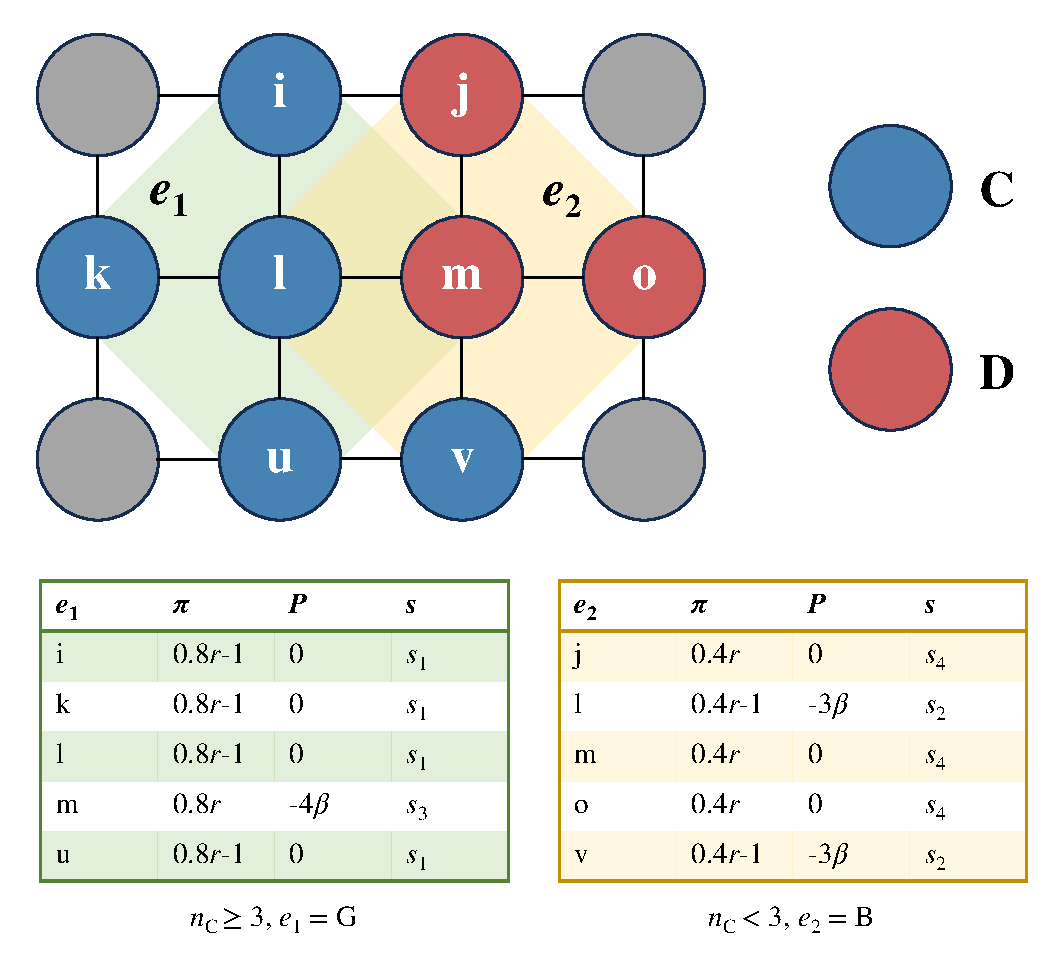
\includegraphics[width=\linewidth]{Fig_1.pdf}
\caption{
Payoff, peer pressure, and state assignment in two overlapping interaction groups for $T=3$. Cooperators are shown in blue and defectors in red; gray sites do not belong to either group. Group $e_1$, centered on $l$, contains $n_{\mathrm{C}}=4\geq T$ cooperators and is a cooperative environment ($\mathrm{G}$), so that its single defector $m$ receives the pressure $-4\beta$. Group $e_2$, centered on $m$, contains $n_{\mathrm{C}}=2<T$ cooperators and is a defective environment ($\mathrm{B}$), so that its two cooperators $l$ and $v$ each receive the pressure $-3\beta$. The tables list the payoff $\pi$ [Eq.~\eqref{eq:payoff}], the peer pressure $P$ [Eq.~\eqref{eq:pressure}], and the state $s$ of every member. Individuals $l$ and $m$ belong to both groups and are in different states in each.
}
\label{fig:Fig1}
\end{figure}

\subsection{Incentives in a single interaction}\label{sec:incentive}

Before turning to the learning dynamics, it is instructive to consider the incentive that Eqs.~\eqref{eq:payoff}--\eqref{eq:effective} create in a single interaction. Suppose that $k\in\{0,\dots,g-1\}$ of the $g-1$ co-players of a focal individual cooperate. The difference between the effective rewards that the focal individual obtains from cooperating and from defecting is
\begin{equation}
\Delta_k=
\begin{cases}
\dfrac{r}{g}-1+\beta k, & k\geq T,\\[1.5ex]
\dfrac{r}{g}-1, & k=T-1,\\[1.5ex]
\dfrac{r}{g}-1-\beta\,(g-1-k), & k\leq T-2.
\end{cases}
\label{eq:delta}
\end{equation}
In the first case the group is cooperative whatever the focal individual does, and defecting would expose it to the pressure of $k$ cooperators. In the second case the focal individual is pivotal: the group is cooperative if it cooperates and defective if it defects, so that it is not pressured either way and only the bare dilemma cost $1-r/g$ remains. In the third case the group is defective whatever the focal individual does, and cooperating would expose it to the pressure of $g-1-k$ defectors.

Equation~\eqref{eq:delta} makes the two-sided nature of the rule explicit. Pressure rewards cooperation only where the co-players already form a cooperative environment, and it penalizes cooperation where they do not. For $T\leq g-1$, unanimous cooperation is a strict Nash equilibrium of the single-group game if $\Delta_{g-1}>0$, i.e., if
\begin{equation}
\beta>\frac{g-r}{g\,(g-1)},
\label{eq:betastar}
\end{equation}
which gives $\beta>0.075$ for $r=3.5$, whereas unanimous defection remains an equilibrium for every $\beta$ as long as $r<g$. Sufficiently strong pressure therefore superimposes a coordination problem on the social dilemma, and for $T\geq2$ increasing $\beta$ also deepens the disadvantage of a lone cooperator, $\Delta_0=r/g-1-\beta(g-1)$. We stress that Eq.~\eqref{eq:delta} describes one-shot incentives only. The Q-learning agents introduced next also value future rewards and, as shown in Sec.~\ref{sec:results}, can sustain cooperation even for $\beta=0$, where $\Delta_k<0$ for all $k$. Equation~\eqref{eq:delta} is therefore used below as a guide for interpreting the simulations, not as a prediction of transition points.

\subsection{Q-learning with action--environment states}\label{sec:qlearning}

Individuals adapt their behavior by Q-learning.\cite{watkins1992qlearning,sutton2018reinforcement} In lattice games the state of a Q-learning agent is commonly identified with its own previous action.\cite{wang2022levy,fan2022incorporating,du2026shaping} Since the effective reward in our model depends on both the action and the environment of the group, we follow Ref.~\onlinecite{li2025environmental} in letting individuals perceive environmental information, and define the state of individual $i$ in a given group as the pair $s=(a_i,e)$ of its current action and the environment of that group. This gives four states,
\begin{equation}
\begin{aligned}
s_1&=(\mathrm{C},\mathrm{G}), & s_2&=(\mathrm{C},\mathrm{B}),\\
s_3&=(\mathrm{D},\mathrm{G}), & s_4&=(\mathrm{D},\mathrm{B}).
\end{aligned}
\label{eq:states}
\end{equation}
Each individual carries its own $4\times2$ table $Q_i(s,a)$, which estimates the discounted cumulative reward of taking action $a\in\mathcal{A}$ in state $s$. Because the environment is defined per group, the same individual is generally in different states in the different groups to which it belongs (see individuals $l$ and $m$ in Fig.~\ref{fig:Fig1}), but it uses a single Q-table in all of them.

In state $s$, an individual selects its action by the $\epsilon$-greedy rule: with probability $1-\epsilon$ it takes the action with the larger value $Q_i(s,a)$, ties being broken at random, and with probability $\epsilon$ it chooses one of the two actions at random. After all members of the group have implemented their actions, individual $i$ receives the effective reward $R_i$ of Eq.~\eqref{eq:effective}, finds itself in the new state $s'$, and updates
\begin{equation}
Q_i(s,a)\leftarrow(1-\alpha)\,Q_i(s,a)+\alpha\Bigl[R_i+\gamma\max_{a'\in\mathcal{A}}Q_i(s',a')\Bigr],
\label{eq:q-learning}
\end{equation}
where $\alpha\in(0,1]$ is the learning rate and $\gamma\in[0,1)$ is the discount factor. Here $s'=(a,e')$ is formed by the action just implemented and the environment $e'$ of the same group after all its members have acted.

\subsection{Simulation procedure}\label{sec:simulation}

Initially, each individual is assigned $\mathrm{C}$ or $\mathrm{D}$ with equal probability, and all Q-values are set to zero. In contrast to the common protocol in which payoffs are accumulated over all overlapping groups before a strategy is updated,\cite{szolnoki2009impact,perc2013evolutionary} we take a single group interaction as the elementary unit of learning. An elementary step consists of the following operations (Algorithm~\ref{alg:PGG_Qlearning}):
(i) a focal individual is selected at random, which defines the interaction group formed by this individual and its four nearest neighbors;
(ii) the environment $e$ of the group is determined from the current actions of its members by Eq.~\eqref{eq:environment}, which fixes the state $s$ of each member;
(iii) each member selects an action by the $\epsilon$-greedy rule, and all five actions are implemented simultaneously;
(iv) the environment $e'$ of the group is re-evaluated, each member receives its effective reward [Eqs.~\eqref{eq:payoff}--\eqref{eq:effective}], and each member updates its Q-table by Eq.~\eqref{eq:q-learning}.
One Monte Carlo step (MCS) comprises $L^2$ elementary steps, so that on average every individual is selected once as the focal individual and takes part in $g=5$ interactions, in each of which it may change its action and updates one entry of its Q-table. Since the action that an individual carries into an interaction is the one it implemented in its most recent interaction, generally in a different group, the state in which it next acts need not coincide with $s'$.

\begin{algorithm}[H]
\caption{Spatial public goods game with environment-dependent peer pressure and Q-learning.}
\label{alg:PGG_Qlearning}
\begin{algorithmic}[1]
\REQUIRE $L$, $r$, $T$, $\beta$, $\alpha$, $\gamma$, $\epsilon$, and the number of Monte Carlo steps $t_{\max}$
\FOR{each individual $i$}
    \STATE Set $a_i$ to $\mathrm{C}$ or $\mathrm{D}$ with equal probability;
    \STATE Set $Q_i(s,a)=0$ for all $s$ and $a$;
\ENDFOR
\FOR{$t=1$ to $t_{\max}$}
    \FOR{$n=1$ to $L^2$}
        \STATE Select a focal individual at random; let $\Omega$ be the group formed by it and its four nearest neighbors;
        \STATE Determine the environment $e$ of $\Omega$ by Eq.~\eqref{eq:environment};
        \FOR{each individual $j\in\Omega$}
            \STATE $s_j\leftarrow(a_j,e)$;
            \STATE With probability $\epsilon$, draw $a'_j$ at random from $\mathcal{A}$; otherwise $a'_j\leftarrow\arg\max_{a}Q_j(s_j,a)$, ties broken at random;
        \ENDFOR
        \STATE Implement all actions simultaneously: $a_j\leftarrow a'_j$ for all $j\in\Omega$;
        \STATE Determine the new environment $e'$ of $\Omega$ by Eq.~\eqref{eq:environment};
        \FOR{each individual $j\in\Omega$}
            \STATE Compute $\pi_j$, $P_j$, and $R_j$ by Eqs.~\eqref{eq:payoff}, \eqref{eq:pressure}, and \eqref{eq:effective};
            \STATE $s'_j\leftarrow(a_j,e')$;
            \STATE Update $Q_j(s_j,a_j)$ by Eq.~\eqref{eq:q-learning};
        \ENDFOR
    \ENDFOR
\ENDFOR
\end{algorithmic}
\end{algorithm}

The quantity of interest is the cooperation level $\rho_{\mathrm{C}}$, the fraction of individuals whose current action is $\mathrm{C}$. Its stationary value is obtained by averaging over the last $10^5$ MCS of runs of $10^6$ MCS. For parameter values at which the system has not become stationary within $10^6$ MCS, the runs are extended to $10^8$ MCS and the average is taken over the last $10^7$ MCS. \AQ{Please state (i) the number of independent realizations over which each data point in Figs.~\ref{fig:Fig2}, \ref{fig:Fig5}, and \ref{fig:Fig6} is averaged and the size of the statistical error, and (ii) the criterion used to decide that a run is not yet stationary, together with the parameter values to which the extension to $10^8$ MCS was applied.} Unless stated otherwise, we use $L=100$, $T=3$, and the learning parameters $\alpha=0.1$, $\gamma=0.9$, and $\epsilon=0.01$, which are typical of related studies.\cite{zhao2024emergence,zheng2024evolution,li2025environmental}


\section{Results and discussion}\label{sec:results}

\subsection{Interplay of pressure intensity and synergy factor}\label{sec:res-r-beta}

\begin{figure*}[t]
\centering
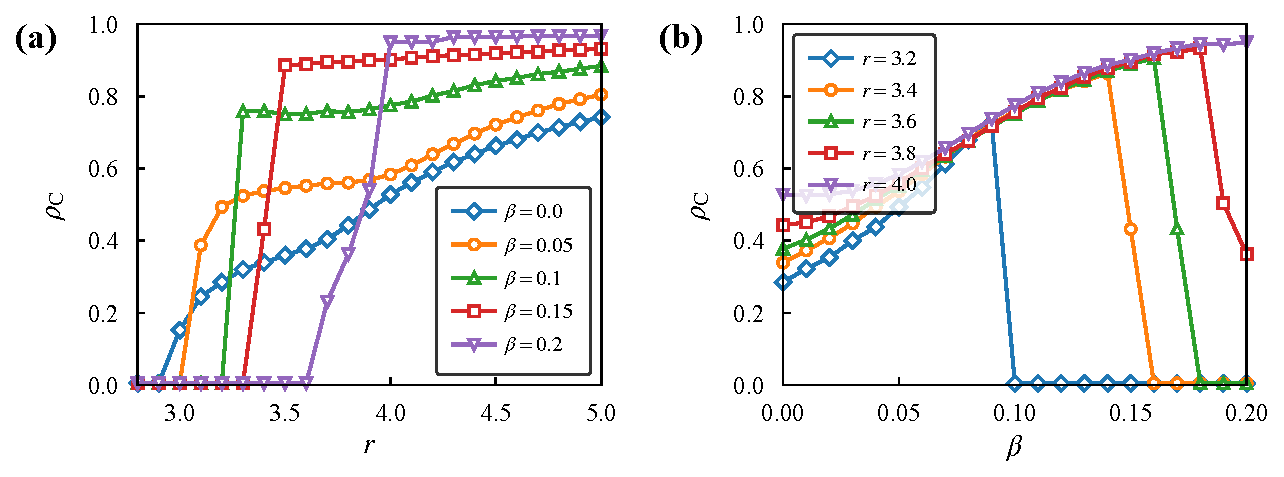
\includegraphics[width=\linewidth]{Fig_2.pdf}
\caption{
Stationary cooperation level $\rho_{\mathrm{C}}$ under environment-dependent peer pressure for the majority threshold $T=3$. (a) $\rho_{\mathrm{C}}$ as a function of the synergy factor $r$ for five pressure intensities $\beta$. (b) $\rho_{\mathrm{C}}$ as a function of $\beta$ for five values of $r$. Increasing $\beta$ raises the cooperation level but shifts the onset of cooperation to larger $r$ and makes it abrupt; at fixed $r<4$, cooperation breaks down once $\beta$ exceeds an $r$-dependent value. Lines are guides to the eye. Other parameters: $L=100$, $\alpha=0.1$, $\gamma=0.9$, and $\epsilon=0.01$.
}
\label{fig:Fig2}
\end{figure*}

We first fix the majority threshold $T=3$ and examine how the stationary cooperation level depends on the synergy factor $r$ and the pressure intensity $\beta$ (Fig.~\ref{fig:Fig2}). Without pressure ($\beta=0$), cooperation emerges continuously near $r\approx3$ and increases smoothly with $r$, reaching $\rho_{\mathrm{C}}\approx0.74$ at $r=5$ [Fig.~\ref{fig:Fig2}(a)]. This baseline is a property of the Q-learning dynamics with the joint state and serves as the reference against which the effect of pressure is measured.

Pressure has two opposing effects. On the one hand, the onset of cooperation moves to larger synergy factors, from $r\approx3.0$ for $\beta=0$ to $r\approx3.3$ for $\beta=0.1$ and $r\approx3.7$ for $\beta=0.2$. In the range $3.0\leq r\leq3.6$, sufficiently strong pressure thus eliminates cooperation that would exist without it. On the other hand, once cooperation is established its level increases with $\beta$: at $r=5$, $\rho_{\mathrm{C}}$ rises from about $0.74$ for $\beta=0$ to about $0.97$ for $\beta=0.2$. The character of the onset changes as well. Whereas $\rho_{\mathrm{C}}$ grows gradually from zero for $\beta=0$, it jumps from zero to $\rho_{\mathrm{C}}\approx0.76$ within a single increment of $r$ for $\beta=0.1$, and to $\rho_{\mathrm{C}}\approx0.88$ within two increments for $\beta=0.15$. For $\beta=0.2$, intermediate values are found for $3.7\leq r\leq3.9$ before a high level of $\rho_{\mathrm{C}}\approx0.95$ is reached at $r=4.0$.

Figure~\ref{fig:Fig2}(b) shows the same behavior as a function of $\beta$. For every $r$ considered, $\rho_{\mathrm{C}}$ first increases monotonically with $\beta$, for example from about $0.29$ to about $0.72$ for $r=3.2$ and from about $0.53$ to about $0.95$ for $r=4.0$. The curves for different $r$ approach one another as $\beta$ grows and nearly coincide for $\beta\gtrsim0.08$. On this cooperative branch the cooperation level is thus controlled mainly by the pressure intensity, whereas the synergy factor determines how far the branch extends. For $r<4$ the branch ends in a breakdown: $\rho_{\mathrm{C}}$ falls to zero at $\beta\approx0.10$, $0.16$, and $0.18$ for $r=3.2$, $3.4$, and $3.6$, respectively, and for $r=3.8$ it has dropped to about $0.36$ at $\beta=0.2$, the largest intensity examined. For $r=4.0$ no breakdown occurs within the examined range. The pressure intensity that maximizes cooperation therefore lies just below the breakdown and increases with $r$.

These opposing effects are consistent with the incentive structure of Eq.~\eqref{eq:delta}. Pressure adds a reward for cooperating in groups that are already cooperative and a penalty for cooperating in groups that are not, so that it reinforces whichever behavior is locally in the majority. A larger synergy factor reduces the bare dilemma cost $1-r/g$ and hence the bias toward defection that the pressure amplifies, which explains why a larger $r$ allows cooperation to withstand stronger pressure. The abrupt onsets are what one would expect if strong pressure made the cooperative and the defective state both self-sustaining. In this respect, the intermediate values of $\rho_{\mathrm{C}}$ observed next to the breakdown [e.g., $\rho_{\mathrm{C}}\approx0.43$ at $(r,\beta)=(3.4,0.15)$] deserve attention. \AQ{Please check whether these intermediate values are stationary states of individual runs or averages over runs that end in different states, and report this; a histogram of final states or a hysteresis and finite-size analysis would settle whether the transition is discontinuous.}

\subsection{Time evolution and spatial organization}\label{sec:res-time}

\begin{figure*}[t]
\centering
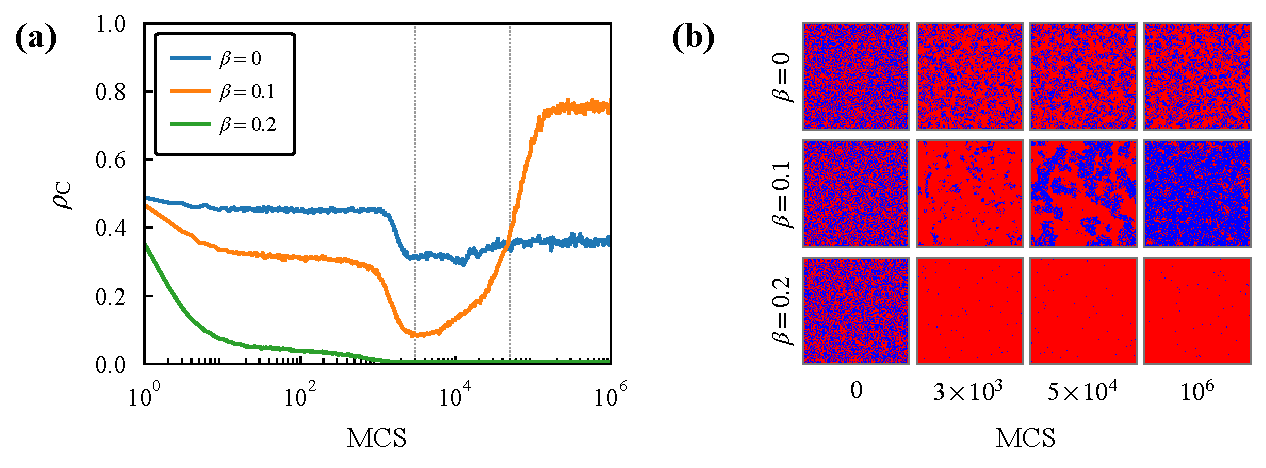
\includegraphics[width=\linewidth]{Fig_3.pdf}
\caption{
Time evolution and spatial organization of cooperation at $r=3.5$ and $T=3$. (a) Cooperation level $\rho_{\mathrm{C}}$ as a function of time (in MCS, logarithmic scale) for $\beta=0$, $0.1$, and $0.2$. The vertical dotted lines mark $t=3\times10^{3}$ and $t=5\times10^{4}$~MCS. (b) Snapshots of the $100\times100$ lattice at $t=0$, $3\times10^{3}$, $5\times10^{4}$, and $10^{6}$~MCS (columns, left to right) for $\beta=0$, $0.1$, and $0.2$ (rows, top to bottom). Cooperators are shown in blue and defectors in red. For each $\beta$, the curve in (a) and the snapshots in (b) are taken from the same run. Other parameters: $\alpha=0.1$, $\gamma=0.9$, and $\epsilon=0.01$.
}
\label{fig:Fig3}
\end{figure*}

To understand how moderate pressure promotes cooperation and strong pressure destroys it, we follow single runs at $r=3.5$ for $\beta=0$, $0.1$, and $0.2$ (Fig.~\ref{fig:Fig3}).

The time series in Fig.~\ref{fig:Fig3}(a) show that cooperation initially declines in all three cases, and the faster the stronger the pressure. Without pressure, $\rho_{\mathrm{C}}$ stays near $0.45$ for about $10^{3}$~MCS, drops to about $0.31$, and settles at $\rho_{\mathrm{C}}\approx0.36$. For $\beta=0.1$, it first decreases to a plateau near $0.31$ and then to a minimum of about $0.09$ at $t\approx3\times10^{3}$~MCS, after which it recovers, overtakes the pressure-free case at $t\approx5\times10^{4}$~MCS, and saturates at $\rho_{\mathrm{C}}\approx0.76$. The pressure that eventually yields the higher cooperation level thus first takes the population through a deeper trough: from the first MCS until $t\approx5\times10^{4}$~MCS, i.e., for more than four decades in time, cooperation is lower with moderate pressure than without. For $\beta=0.2$, $\rho_{\mathrm{C}}$ falls to about $0.05$ within $10^{2}$~MCS, vanishes by about $10^{3}$~MCS, and does not recover. The relaxation is slow in all cases in which cooperation survives, the stationary state being reached only after about $10^{5}$~MCS.

The snapshots in Fig.~\ref{fig:Fig3}(b) show how these trajectories are organized in space. Without pressure, cooperators and defectors remain finely intermixed at all times. For $\beta=0.1$, the cooperators that survive the initial decline are concentrated in a few compact clusters at $t=3\times10^{3}$~MCS. By $t=5\times10^{4}$~MCS these clusters have grown into large domains, and at $t=10^{6}$~MCS cooperators occupy most of the lattice, with defectors scattered among them. Notably, at $t=5\times10^{4}$~MCS the cooperation levels for $\beta=0$ and $\beta=0.1$ are nearly equal, yet the spatial arrangements differ qualitatively: a fine-grained mixture in the former case and segregated domains in the latter. For $\beta=0.2$, the lattice is already almost entirely defecting at $t=3\times10^{3}$~MCS, and only isolated cooperators appear thereafter, as expected from the exploration rate $\epsilon$. Moderate pressure therefore promotes cooperation by stabilizing and expanding compact cooperative domains, in line with the reinforcement of the local majority implied by Eq.~\eqref{eq:delta}, whereas strong pressure removes cooperators before such domains can form.

\subsection{State-resolved learning dynamics}\label{sec:res-learning}

\begin{figure*}[t]
\centering
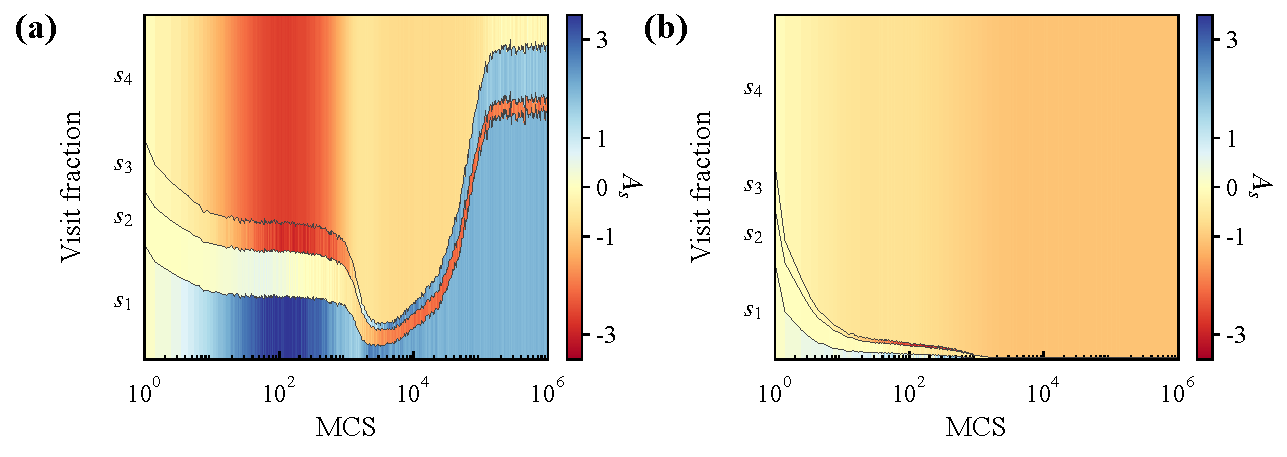
\includegraphics[width=\linewidth]{Fig_4.pdf}
\caption{
State-resolved learning dynamics at $r=3.5$ and $T=3$ for (a) $\beta=0.1$ and (b) $\beta=0.2$. The four bands, stacked from bottom to top in the order $s_1=(\mathrm{C},\mathrm{G})$, $s_2=(\mathrm{C},\mathrm{B})$, $s_3=(\mathrm{D},\mathrm{G})$, and $s_4=(\mathrm{D},\mathrm{B})$, show the fractions of visits to the four states as functions of time (in MCS, logarithmic scale); the vertical extent of a band is its visit fraction, and the four fractions sum to one. The color of each band gives the action-value gap $A_s(t)$ of Eq.~\eqref{eq:gap}, with blue (red) indicating a preference for cooperation (defection) in that state. Note the nonlinear color scale. Other parameters: $\alpha=0.1$, $\gamma=0.9$, and $\epsilon=0.01$.
}
\label{fig:Fig4}
\end{figure*}

The spatial picture can be connected to what the agents learn. For each state $s$ we record the fraction of visits it receives in each MCS and the action-value gap
\begin{equation}
A_s(t)=\bigl\langle Q_i(s,\mathrm{C})-Q_i(s,\mathrm{D})\bigr\rangle_{s,t},
\label{eq:gap}
\end{equation}
where $\langle\cdot\rangle_{s,t}$ denotes the average over all visits to state $s$ during MCS $t$. The Q-values are evaluated before the corresponding update, and repeated visits by the same individual are counted separately. A positive (negative) $A_s$ means that, on average, the agents visiting state $s$ prefer cooperation (defection) there. Figure~\ref{fig:Fig4} shows both quantities for the runs of Fig.~\ref{fig:Fig3} with $\beta=0.1$ and $\beta=0.2$.

Under moderate pressure [Fig.~\ref{fig:Fig4}(a)], $A_{s_1}$ becomes strongly positive within the first $10^{2}$~MCS: cooperators in cooperative groups quickly learn to keep cooperating. In the same period, $A_{s_4}$ and $A_{s_3}$ become negative, so that defectors initially learn to keep defecting in either environment, which corresponds to the plateau of $\rho_{\mathrm{C}}$ in Fig.~\ref{fig:Fig3}(a). Although visits concentrate in $s_4$ as cooperation approaches its minimum, the states $s_1$ and $s_3$ never disappear, because the surviving clusters of Fig.~\ref{fig:Fig3}(b) continue to provide cooperative environments. In these environments defectors are pressured and cooperators are not, and $A_{s_3}$ eventually changes sign: defectors that find themselves in a cooperative group now prefer to switch to cooperation. From this point on, cooperative environments expand and the share of $s_1$ grows until it accounts for the majority of visits. In the stationary state, $A_{s_1}$ and $A_{s_3}$ are positive, whereas $A_{s_2}$ is negative and $A_{s_4}$ remains weakly negative. The agents have thus learned an environment-conditional rule, namely to cooperate in cooperative groups and to defect in defective ones, largely irrespective of their own previous action. In other words, they have learned to conform to the local environment, and the stationary cooperation level reflects the fraction of groups that this rule keeps cooperative.

Under strong pressure [Fig.~\ref{fig:Fig4}(b)], visits collapse onto $s_4$ within about $10^{2}$~MCS, and the shares of $s_1$, $s_2$, and $s_3$ vanish before $10^{3}$~MCS. Because all Q-values start from zero, the earliest updates are governed by the immediate rewards. According to Eq.~\eqref{eq:delta}, at $\beta=0.2$ a cooperator with at most one cooperating co-player loses an additional $0.6$ to $0.8$ relative to defecting, which is roughly two to three times the bare dilemma cost $1-r/g=0.3$. Cooperators in defective groups therefore abandon cooperation rapidly, which turns further groups defective and exposes their remaining cooperators to the same pressure. The states $s_1$ and $s_3$ are then visited so rarely that the preference of defectors for switching to cooperation in cooperative environments ($A_{s_3}>0$), which under moderate pressure takes more than $10^{3}$~MCS to develop, cannot be learned, while $A_{s_4}$ remains negative throughout. Strong pressure thus does not make cooperation unprofitable where cooperative environments exist; according to Eq.~\eqref{eq:delta} it makes cooperation more profitable there. Rather, it eliminates those environments before the agents can learn to exploit them.

\subsection{Role of the environmental threshold}\label{sec:res-threshold}

\begin{figure*}[t]
\centering
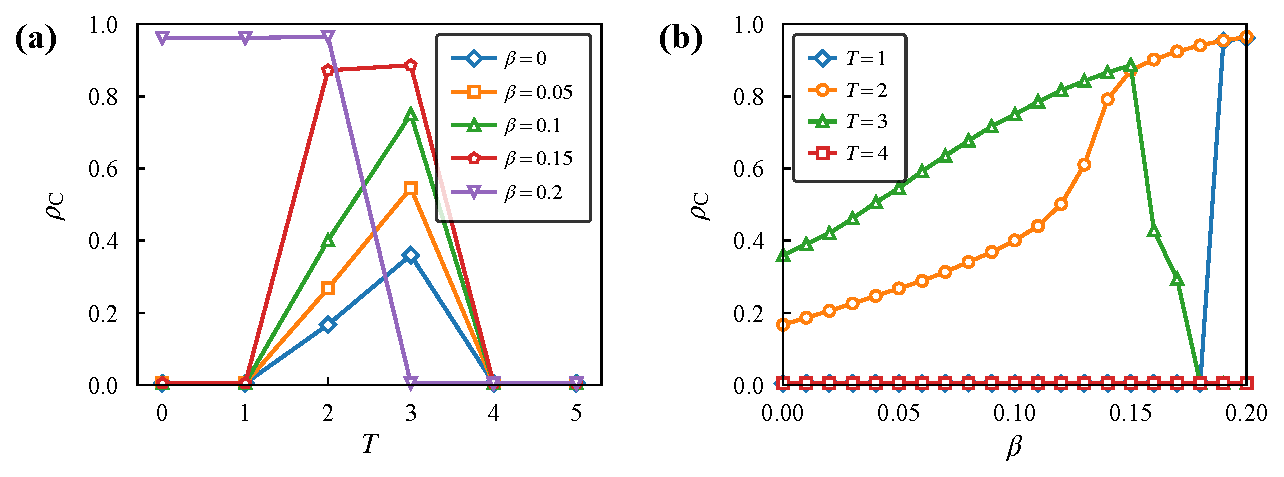
\includegraphics[width=\linewidth]{Fig_5.pdf}
\caption{
Effect of the environmental threshold $T$ at $r=3.5$. (a) Stationary cooperation level $\rho_{\mathrm{C}}$ as a function of $T$ for five pressure intensities $\beta$. For $T=0$ every group is classified as cooperative, and for $T=5$ only fully cooperating groups are. (b) $\rho_{\mathrm{C}}$ as a function of $\beta$ for $T=1$, $2$, $3$, and $4$. Lines are guides to the eye. Other parameters: $L=100$, $\alpha=0.1$, $\gamma=0.9$, and $\epsilon=0.01$.
}
\label{fig:Fig5}
\end{figure*}

We now vary the threshold $T$ at $r=3.5$ (Fig.~\ref{fig:Fig5}). Figure~\ref{fig:Fig5}(a) shows that the threshold that maximizes cooperation depends on the pressure intensity. For weak and moderate pressure ($\beta\leq0.15$), cooperation is highest at the majority threshold $T=3$, followed by $T=2$, and is absent for all other thresholds. For $\beta=0.2$ the situation is reversed: cooperation is absent at $T=3$ but reaches $\rho_{\mathrm{C}}\approx0.96$ for $T\leq2$. For $T=4$ and $T=5$, cooperation is absent at every $\beta$ examined.

The dependence on $\beta$ at fixed $T$ [Fig.~\ref{fig:Fig5}(b)] can be understood from Eq.~\eqref{eq:delta}. For $T=1$, cooperators are never pressured and the sanction on defectors, $-\beta n_{\mathrm{C}}$, is weak wherever cooperators are scarce. Cooperation remains absent up to $\beta=0.18$ and then jumps to $\rho_{\mathrm{C}}\approx0.96$ at $\beta=0.19$: only strong pressure on defectors can by itself outweigh the dilemma cost. For $T=2$, two cooperators suffice to make a group cooperative, and a cooperator is pressured only if it is alone in its group. Cooperation then increases monotonically with $\beta$, from about $0.17$ to about $0.96$, most steeply for $0.12\leq\beta\leq0.15$, and no breakdown occurs. For $T=3$, the cooperation level is higher than for $T=2$ up to its maximum of about $0.88$ at $\beta=0.15$, but it then decreases and vanishes at $\beta=0.18$ through the mechanism analyzed in Secs.~\ref{sec:res-time} and \ref{sec:res-learning}. For $T=4$, the cooperation-favoring case of Eq.~\eqref{eq:delta} requires all four co-players to cooperate, whereas cooperators are pressured whenever at most two of their co-players cooperate, i.e., in most mixed groups. Pressure can then essentially only harm cooperation, which remains absent. A lower threshold thus protects cooperators from pressure and removes the breakdown, at the price of a weaker benefit at small $\beta$; a higher threshold exposes cooperators to pressure in ever more configurations.

It is important to note that the threshold also matters without any pressure: at $\beta=0$, $\rho_{\mathrm{C}}\approx0.17$ for $T=2$ and $\rho_{\mathrm{C}}\approx0.36$ for $T=3$, whereas cooperation is absent for all other thresholds [Fig.~\ref{fig:Fig5}(a)]. Since the payoffs at $\beta=0$ do not depend on $T$, this difference arises entirely from the way in which the threshold partitions the experience of the agents into states. For $T=0$ every group is classified as cooperative, so that the state carries no environmental information at all. The threshold therefore plays two roles in the present model: it decides who is pressured, and it decides which situations the agents can tell apart. The two roles cannot be separated in Fig.~\ref{fig:Fig5}; the majority threshold appears to combine an informative partition of the states with a balanced allocation of pressure.

\subsection{Comparison with environment-independent pressure and reduced state representations}\label{sec:res-comparison}

\begin{figure*}[t]
\centering
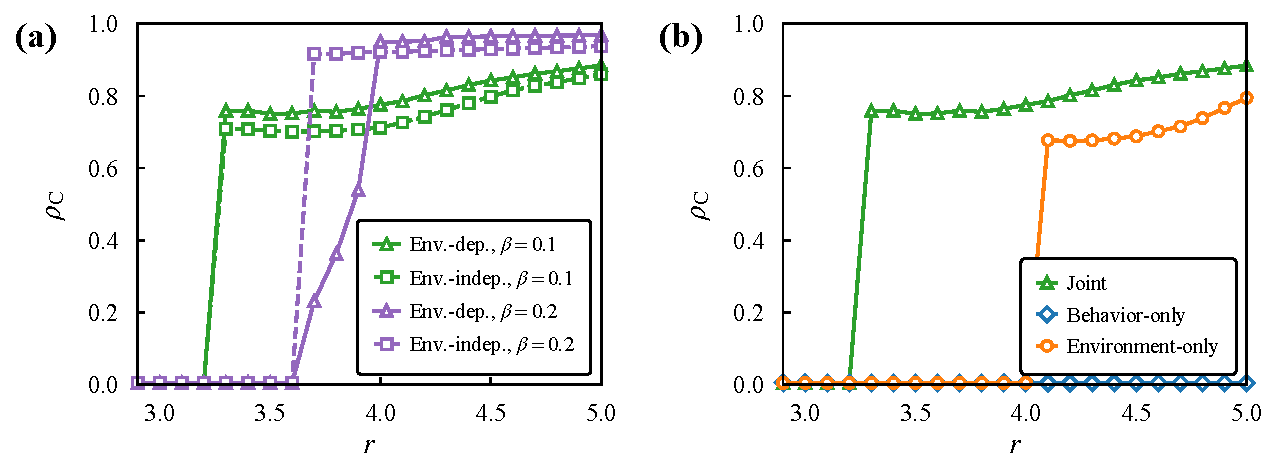
\includegraphics[width=\linewidth]{Fig_6.pdf}
\caption{
Comparison of pressure rules and state representations for $T=3$. (a) Stationary cooperation level $\rho_{\mathrm{C}}$ as a function of $r$ under environment-dependent pressure [Eq.~\eqref{eq:pressure}, solid lines] and environment-independent pressure [Eq.~\eqref{eq:indep}, dashed lines] for $\beta=0.1$ and $\beta=0.2$; both rules use the joint state $(a_i,e)$. (b) $\rho_{\mathrm{C}}$ as a function of $r$ under environment-dependent pressure with $\beta=0.1$ for three state representations: the joint state $(a_i,e)$, a behavior-only state $a_i$, and an environment-only state $e$. Lines are guides to the eye. Other parameters: $L=100$, $\alpha=0.1$, $\gamma=0.9$, and $\epsilon=0.01$.
}
\label{fig:Fig6}
\end{figure*}

Finally, we assess the two ingredients of the model separately, by replacing either the pressure rule or the state representation while keeping the action set and the learning parameters unchanged (Fig.~\ref{fig:Fig6}).

\paragraph*{Pressure rule.}
As a reference we consider an environment-independent rule under which every individual is pressured by all group members who hold the opposite action, regardless of the environment,
\begin{equation}
P_i^{\mathrm{ind}}=
\begin{cases}
-\beta\,n_{\mathrm{D}}, & a_i=\mathrm{C},\\
-\beta\,n_{\mathrm{C}}, & a_i=\mathrm{D},
\end{cases}
\label{eq:indep}
\end{equation}
which is in the spirit of the mutual punishment studied in Ref.~\onlinecite{yang2015peer}. The states are still defined by Eq.~\eqref{eq:states} with $T=3$, so that only the reward differs between the two rules. Figure~\ref{fig:Fig6}(a) shows that neither rule is uniformly superior. For $\beta=0.1$, cooperation sets in at the same synergy factor, $r\approx3.3$, under both rules, and the environment-dependent rule yields a slightly higher level throughout (e.g., $\rho_{\mathrm{C}}\approx0.76$ against $0.71$ at $r=3.3$). For $\beta=0.2$, the environment-independent rule reaches $\rho_{\mathrm{C}}\approx0.92$ already at $r=3.7$, whereas the environment-dependent rule attains a comparable level only at $r=4.0$, beyond which it is again slightly higher.

The single-interaction incentive explains this pattern. For the rule of Eq.~\eqref{eq:indep}, the counterpart of Eq.~\eqref{eq:delta} is
\begin{equation}
\Delta_k^{\mathrm{ind}}=\frac{r}{g}-1+\beta\,(2k-g+1),
\label{eq:delta-indep}
\end{equation}
because a change of action both removes the pressure from one side and incurs that from the other. For $g=5$ and $T=3$ the two rules create identical incentives for $k=0$, $2$, and $4$, but they differ for $k=1$ and $k=3$, where the pressure term is $\mp3\beta$ under the environment-dependent rule and $\mp2\beta$ under the environment-independent rule. By exempting the local majority from pressure, the environment-dependent rule sharpens the incentive to follow the majority on both sides of the threshold. This helps cooperation where cooperative groups are common, which accounts for the higher level on the cooperative branch, and it hurts cooperation where they are rare, which accounts for the larger synergy factor required under strong pressure.

\paragraph*{State representation.}
Figure~\ref{fig:Fig6}(b) compares the joint state with two reduced representations under environment-dependent pressure with $\beta=0.1$. With the behavior-only state, in which the agents distinguish only their own action, cooperation is absent over the entire range $r\leq5$. With the environment-only state, in which they distinguish only $\mathrm{G}$ from $\mathrm{B}$, cooperation appears at $r\approx4.1$ with $\rho_{\mathrm{C}}\approx0.68$ and reaches about $0.80$ at $r=5$. With the joint state, cooperation appears already at $r\approx3.3$ and is higher at every $r$. Under these conditions, environmental information is thus the more important of the two components. This is consistent with the absence of cooperation for $T=0$ and $\beta\leq0.15$ in Fig.~\ref{fig:Fig5}(a), where every group is classified as cooperative and the joint state reduces to the behavior-only one. This is plausible, because under Eq.~\eqref{eq:pressure} the consequence of an action depends on the environment, and an agent that cannot perceive the environment cannot learn the conditional rule identified in Sec.~\ref{sec:res-learning}. Knowledge of one's own action adds to this, because the joint state allows agents to learn separately whether to maintain or to change their behavior in a given environment. We note that this comparison was made for a single pressure intensity and threshold; whether the ordering of the three representations holds more generally remains to be tested.


\section{Conclusion}\label{sec:conclusion}

We have studied a spatial public goods game in which peer pressure depends on the local environment: groups with at least $T$ cooperators sanction their defectors, and groups with fewer cooperators sanction their cooperators. Individuals adapt by Q-learning with a state that comprises their own action and the environment of the group in which they currently interact.

Our main finding is that such pressure is double-edged. For the majority threshold, increasing the pressure intensity raises the cooperation level wherever cooperation survives, but it also raises the synergy factor needed for cooperation to appear and turns its gradual emergence into an abrupt one. At a fixed synergy factor, cooperation therefore increases with the pressure intensity up to a breakdown point, which moves to stronger pressure as the synergy factor grows. The time-, space-, and state-resolved dynamics explain this behavior. Under moderate pressure, compact cooperative clusters survive an initial decline, and within them agents learn to cooperate whenever their group is cooperative and to defect otherwise, i.e., to conform to the local environment; the clusters then expand. Under strong pressure, cooperative environments disappear before this conditional preference can be learned. An analysis of the incentives in a single interaction supports this interpretation: environment-dependent pressure rewards cooperation in cooperative groups and penalizes it in defective ones, and thereby superimposes a coordination problem on the social dilemma.

Two further results qualify this picture. First, the environmental threshold reshapes the response to pressure. Low thresholds protect cooperators from pressure and avoid the breakdown, but they are effective only under strong pressure; the majority threshold is the most favorable under weak and moderate pressure; and high thresholds suppress cooperation at all intensities. Second, neither ingredient of the model is beneficial unconditionally. Environment-dependent pressure yields slightly more cooperation than environment-independent pressure where cooperation is established, but it requires a larger synergy factor when the pressure is strong. The joint action--environment state sustains cooperation over a wider range of synergy factors than either of its components, of which the environmental one is the more important.

Several limitations should be kept in mind. The results were obtained for a single lattice size and interaction topology, for one set of learning parameters, and for random initial conditions with equal numbers of cooperators and defectors. Since strong pressure favors whichever behavior is locally in the majority, the outcome can be expected to depend on the initial fraction and spatial arrangement of cooperators, and the abrupt transitions call for an analysis of hysteresis and finite-size effects. The threshold simultaneously determines the allocation of pressure and the information available for learning, and the two effects could be disentangled by assigning them separate thresholds. Finally, pressure is costless for those who exert it and linear in their number, in contrast to costly punishment.\cite{fehr2002altruistic,chen2014probabilistic} Relaxing these assumptions, and extending the model to heterogeneous interaction networks and hypergraphs,\cite{shi2024model} heterogeneous learning parameters,\cite{lee2025granular} and alternative definitions of states and state transitions,\cite{guo2022effect} are natural directions for future work. More generally, our results suggest that the effect of social feedback on cooperation cannot be assessed independently of the local conditions under which it is applied and of how individuals learn from it.


\begin{acknowledgments}
\AQ{Add funding information here (funding agency and grant numbers); AIP journals have no separate ``Funding'' section.}
The authors used OpenAI Codex (GPT-6.1 Sol) to assist with the preparation of the manuscript and with the development of the simulation and plotting code. The authors reviewed and edited all such output and take full responsibility for the content of this article. \AQ{Please verify the exact name and version of every generative-AI tool used, make sure that this statement covers all of them and all of their uses, and check it against the current AIP Publishing policy on AI tools before submission.}
\end{acknowledgments}

\section*{Author Declarations}

\subsection*{Conflict of Interest}
The authors have no conflicts to disclose.

\subsection*{Author Contributions}
\AQ{List the contribution of each author using the CRediT taxonomy, e.g., ``\textbf{First Author}: Conceptualization (equal); Methodology (lead); Software (lead); Writing -- original draft (lead). \textbf{Corresponding Author}: Conceptualization (equal); Supervision (lead); Writing -- review \& editing (lead).''}

\section*{Data Availability}
The data that support the findings of this study are available from the corresponding author upon reasonable request.

% The AIP substyle of REVTeX suppresses the heading of the reference list.
\renewcommand{\bibsection}{\section*{References}}
% No \bibliographystyle here: REVTeX selects the AIP numerical style itself
% (aipnum4-2.bst), and the `article-title' class option only takes effect
% when the style is left to the class.
\bibliography{ref}

\end{document}
